\section{Mercados Financieros}

El mercado financiero es un espacio con marco institucional que permite poner
en contacto a oferentes y demandantes para que efectúen transacciones
financieras. La idea de mercado como foro organizado a la que acuden agentes
económicos para efectuar transacciones queda reducida en el mundo financiero
como las bolsas de valores \cite{mishkin2006financial}.

El concepto de mercado financiero se utiliza en general para referirse a
cualquier mercado organizado en el que se negocien instrumentos financieros de
todo tipo, como acciones, divisas, etc. El espacio para generar estas
interacciones no necesariamente debe ser físico. Por otro lado, el negociar
instrumentos financieros implica a grandes rasgos: definir su precio e
intercambiarlos, por ende, estos mercados están basados en las fuerzas de
oferta y demanda, ubicando a todos los oferentes en el mismo lugar, y así
facilitarle la búsqueda a los demandantes. Dentro de este tipo de mercado se
distinguieron bloques de estudio en la economía moderna
\cite{jensen1984theory}.

Una de las razones que hace importante este tipo de mercado, es su
funcionalidad, ya que permiten: por un lado aumentar el capital, siendo esto
uno de los casos favorables, ya que también hay probabilidades considerables de
disminuir el capital; comercio internacional, como en los mercados de divisas,
por ejemplo Forex; y reunir a quienes necesitan recursos financieros, con los
que tienen recursos financieros. Factores que permiten generar los efectos de
oferta y demanda.

En este tipo de mercado se definen los siguientes términos
\cite{nevmyvaka2003electronic}:
\begin{itemize}
    \item \emph{Dealer}: Un dealer es un ente presente en los mercados que está
    dispuestos a comprar o vender.
    \item \emph{Orders}: Operación de compra/venta de activos.
    \item \emph{Bid price}: Precio al cual un \emph{dealer} está dispuesto a
    comprar.
    \item \emph{Ask price}: Precio al cual un \emph{dealer} está dispuesto a
    vender.
    \item \emph{Market orders}: instrucción del cliente al dealer, de comprar o
    vender al mejor precio posible dentro de los valores actuales del mercado.
    Esto asegura la realización de la transacción, pero no el precio.
    \item \emph{Limit orders}: es una orden para comprar a un valor máximo
    (precio determinado), o para vender a un valor mínimo (precio determinado).
    Esto le da al cliente el control sobre el precio al que se ejecuta el
    comercio, sin embargo, no garantiza la realización de la transacción.
\end{itemize}

El conjunto de \emph{Limit orders} forman los \emph{books} para cierto
instrumento, los cuales proveen información detallada del mismo. Con estos
datos se forman los llamados bid-ask spreads, que es la diferencia entre el
precios cotizados para una venta inmediata (oferta) y una compra inmediata
(bid).  También se generan los bid-ask qoute, el cual define cotas para el
precio de transacción.

\subsection{Mercados bursátiles}
Los mercados bursátiles están clasificados dentro de los mercados de capitales,
en donde se negocian activos financieros. Este tipo de mercado provee
financiamiento por medio de la emisión de acciones y permiten luego el
intercambio de estas. La aplicación más directa de este tipo de mercados, son
las bolsas de valores, cuyo origen se remonta a finales del siglo XV en las
ferias medievales de Europa. Las bolsas de valores se pueden definir como
mercados organizados y especializados, en los que se pueden realizar
transacciones de títulos de valores por medio de intermediarios autorizados.
Estas bolsas ofrecen al público y a sus miembros facilidades, mecanismos e
instrumentos técnicos que facilitan la negociación de títulos de valores
susceptibles de ofertas públicas, y precios determinados mediante subasta
\cite{levine1998stock}.

La principal función de las Bolsas de Valores es proporcionar a los
participantes información objetiva, completa y permanente de los valores y las
empresas inscritas en la bolsa, sus emisiones y las operaciones que en ella se
realicen. Además debeb supervisar las actividades. Las componentes de este
sistema son los activos y las instituciones financieras, cuya misión es
contactar demandantes y oferentes en los mercados donde se negocian los
diferentes instrumentos o activos financieros. En el documento se hablará de
instrumento, ya que pueden ser acciones, divisas, etc. los cuales quedan
generalizados bajo ese concepto.

%La economía presenta a este tipo de mercado, como de competencia perfecta, ya
%que sus características principales son: elevado número de compradores y
%vendedores; La decisión individual de cada uno de ellos ejercerá escasa
%influencia sobre el mercado global; Homogeneidad de los productos, es decir, no
%existen diferencias entre productos que venden los oferentes; Transparencia del
%mercado, todos los participantes tienen pleno conocimiento de las condiciones
%generales en que opera el mercado; Libertad de entrada y salida de empresas,
%todos los participantes, cuando lo deseen, podrán entrar o salir del mercado a
%costos nulos o casi nulos \cite{mankiw2011principles}. 
%
%Por otra parte, Fama propuso la Hipótesis de eficiencia de los mercados
%\cite{malkiel2012efficient}, la cual establece que los mercados son eficientes
%cuando son capaces de trasladar a los precios de los instrumentos financieros,
%todos los datos relevantes, por lo tanto, el precio refleja \emph{toda} la
%información disponible, y lo hace de manera insesgada. Cuando se cumplen estas
%condiciones, el precio del instrumento financiero se comporta como un
%\emph{Random Walk} \cite{fama1965random}, por lo que los resultados no pueden
%ser predichos sistemáticamente.

%TODO
\subsection{Mercado de divisas}
El mercado de divisas también conocido como Forex(abreviatura del término
inglés Foreign Exchange) es un mercado de intercambio de divisas extranjeras.

La base de este mercado es beneficiarse con las fluctuaciones presentadas entre
una moneda frente a otra tomando una posición de compra o venta dependiendo si
se especula que se va a ganar o perder valor entre la relación de dichas
monedas. La compra y venta por los acontecimientos económicos y políticos
presentados en cada país se denomina reactiva, mientras que la compra y venta
en acontecimientos anticipados se denomina especulativa. 

Las monedas se cotizan en pares, tales como EUR/USD o USD/JPN. La moneda que
está de primer se le dice moneda base y la segunda es la moneda en contra. En
cuanto a su manejo, por ejemplo en un par EUR/USD el trader cree que la
economía americana se va a debilitar, se lastimaría el dólar y por lo tanto se
haría una compra de EUR/USD esperando que el euro se aprecie frente al dólar
estadounidense. 

Algunas de las características principales son:
\begin{itemize}
 \item Forex no tiene ubicación física, todo funciona a través de las redes de
 los bancos, es decir, que a través de las transacciones entre Bancos, empresas
 y personas se compra y vende un par de divisas.
 \item Disponibilidad las 24 horas del día gracias a la diferencia de horarios
 entre países. Este inicia todos los días en Sídney, después en Tokio, Londres
 y Nueva York.
 \item Uso de plataformas por internet.
\end{itemize}

Existen varias plataformas web (software) para para acceder a Forex, y cada uno
están regulados por distintas entidades. Para esta memoria se utilizarán datos
financieros del mercado de divisas.

\section{Series de tiempo financiera}

La mayoría de los fenómenos que se estudian en su componente temporal, deben
tomar en cuenta la dinámica de los proceso con la finalidad tener una
comprensión general del mismo. Una herramienta útil en dicho objetivo es el
análisis de series de tiempo. Una serie de tiempo, es una secuencia de datos
indexados por su marca temporal. Se pueden presentar casos de series de tiempo
en una multitud de disciplinas como ingeniería, sociología, economía, finanzas
por solo mencionar algunas de ellas.

El propósito fundamental es mostrar las técnicas que permitan hacer inferencias
del proceso en estudio incluyendo su predicción. Esto se logra estableciendo
modelos probabilísticos hipotéticos que representen a los datos; y en
consecuencia, se lleva a cabo el proceso de ajuste, que incluye desde la
estimación hasta la predicción, una vez que se ha determinado un modelo
satisfactorio para la muestra de datos \cite{box2011time}
\cite{vandaele1983applied}. 
%Los modelos de series deben considerar la
%naturaleza del fenómeno y determinar los factores que pueden ser incluidos en
%el.

En particular, el análsis de una serie de tiempo financiera puede enfocarse en
analizar de forma teórica y práctica la valoración de cierto instrumento en el
tiempo, como también los volúmenes transados, etc. Lo que se intenta es modelar
la incertidumbre generada por las características propias de este fenómeno
\cite{tsay2005analysis}. 

Las características diferenciadoras han propiciado numerosos trabajos en las
áreas de econometría y economía financiera desde los años 60. Es por ello que,
en el área financiera las evidencias sobre patrones ha conducido a la
formulación de distintos modelos matemáticos.

%TODO: Revisar
\subsection{Descripción de serie financiera}

Una tendencia en el análisis de las series financieras, es el seguimiento del
precio de un instrumento en el tiempo.
%Las series de tiempo financieras, se basan en el estudio del precio de un
%instrumento financiero en el tiempo. 
Existen varios tipos de precios que se pueden analizar, por un lado están los
indicadores que se utilizaron en los primeros estudios formales, los cuales
mostraban información al respecto de los precios de: \emph{apertura},
\emph{cierre}, \emph{el más bajo}, \emph{el más alto}, \emph{promedio}. Esos
datos estaban orientados a tomar métricas respecto a valores que resumían los
cambios de precio de un instrumento en un día. Una muestra gráfica de esta
información se puede ver en la figura \ref{fig:microsoft} \footnote{Imagen
tomada de \url{http://www.stockrageous.com/}}
%con estos datos quedaban gráficos como el siguiente:

\begin{figure}[h!t]
    \begin{center}
        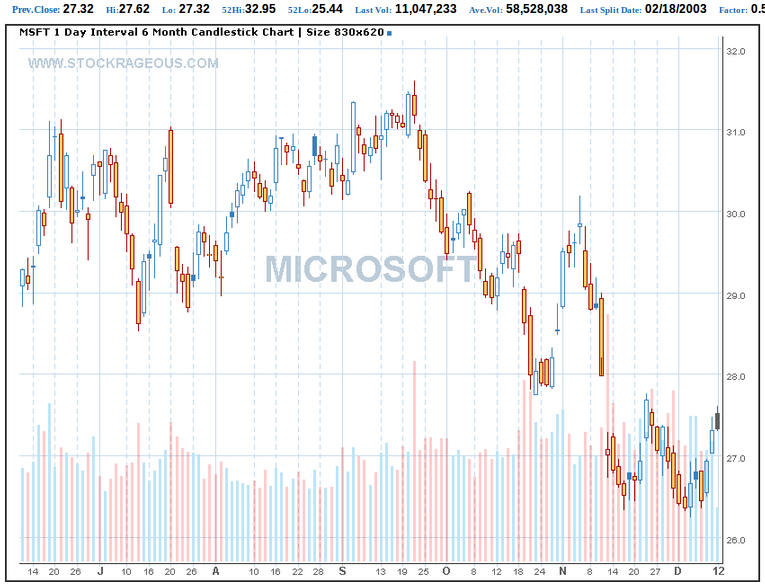
\includegraphics[width=0.5\textwidth]{images/microsoft}
        \caption{Información de los precios de microsoft en la bolsa.}
        \label{fig:microsoft}
    \end{center}
\end{figure}

Con esa información se realizaban \emph{estudios técnicos}
\cite{taylor1992use}, los cuales proporcionaban pronósticos de tendencias (como
subir o bajar de precio), basándose en la inspección visual y búsqueda de
patrones en los precios anteriores del instrumento. 

Sin embargo la data estudiada actualmente corresponde a data \emph{intra
diaria}, la cual reside en los valores específicos en que se compró o vendió
algún instrumento.  Ese precio se conoce como el \emph{last price}, y
corresponde al valor específico con el cual se realizó la transacción. La forma
de como se efecúa este evento es mediante los \emph{market} o \emph{limit
orders}, donde existe una cola de compras o ventas obtenidas mediante los
\emph{limit orders} y que cuando se cumpla la condición asociada (de vender o
comprar a cierto precio), se realiza la transacción y se registra dicho
\emph{last price}. Recopilando esa información, se puede generar una secuencia
temporal de los \emph{last prices}. 
%Estudios prácticos de estas series \cite{biais2012empirical},
%generalizan su gráfica con forma de \emph{U},

A través de la historia, estas interacciones se realizaban personalmente en las
bolsas de comercio, en los llamados \emph{floor market}
\cite{jain2005financial}, sin embargo con el avance de las tecnologías, se han
implementado distintas plataformas de \emph{trading electrónico}: un método de
negociación de instrumentos financieros por medios electrónicos
\cite{weston2002electronic}. Estas tecnologías se utilizan para reunir a
compradores y vendedores a través de plataformas de comercio electrónico, como
por ejemplo: National Association of Securities Dealers Automated Quotation
(NASDAQ), New York Stock Exchange (NYSE), etc. Tomando en cuenta las nuevas
frecuencias de aparición de datos, en el orden de fracción de segundos, se
torna difícil manejar los datos de forma humana, es por esta razón que es
necesario realizar análisis cuantitativos mediante algoritmos computacionales.

%Las series financieras de alta frecuencia tienen características particulares
%en relación a otras series, como son: 
%\begin{itemize}
%	\item Frecuencia: la frecuencia en la observación de los datos es mayor que
%en otro tipo de series de tiempo, en el orden de fracción de segundos.
%	\item Heterocedasticidad: ocurre cuando la varianza de las perturbaciones
%no es constante a lo largo de las observaciones.  Este factor hace inadecuados
%los modelos desarrollados para series estacionarias.
%	\item No estacionalidad: en muchos casos la media y varianza se presentan
%como no estacionarias.
%	\item Información oculta: se pueden encontrar distintos tipos de patrones a
%diferentes niveles de escala.
%\end{itemize}

%TODO:
\subsection{Serie de tiempo Forex}

\section{High Frequency Trading}

Esta sección busca detallar componentes de un sistema de trading electrónico, 
conceptos de funcionamientos, actores, etc.

\subsection{Sistema de trading y compoenentes}
Un sistema electrónico de trading es una infraestructura que permite el ingreso
de órdenes, generación y envío de datos financieros con precios, y el match de
dichas órdenes en base a un criterio predefinido.

Una de las ventajas de este tipo de sistema por sobre sus antecesores, es su
diseño robusto, ya que permiten automatizar el proceso, entregar confiabilidad,
escalabilidad, seguridad y performance: capacidades que luego de cierto volumen
de son imposibles de realizar de forma manual.

No existe una estructura estándar en los distintos mercados mundiales para
sistemas de trading, generalmente se emplea una arquitectura compuesta por los
siguientes elementos:
\begin{itemize}
 \item Interfaz de ingreso de órdenes del lado del servidor, la cual implementa
un protocolo propietario o estándar.
 \item Terminales de trading, con un \emph{trader} humano operando u otros
sistemas, que se comunican mediante cierto protocolo y se conecta a la
interfaz. Estas son conocidas como frontend si el usuario es una persona, o un
Order Management System (OMS).
 \item Matching Engine, el cual recibe órdenes de compra y venta según un
criterio predefinido las empareja, juntando así compradores y vendedores de un
mismo activo que se ponen de acuerdo en un precio y una cantidad.
 \item Interfaz de Market Data, que presenta los precios disponibles en el
sistema como referencia, e informa de nuevas operaciones realizadas, a la que
se conectan distintos \emph{vendors} de data y las terminales y sistemas antes
mencionados.
 \item Sistema de \emph{backoffice} para hacer seguimiento de las operaciones
concertadas, la realización de \emph{allocations} o \emph{giveups}, si el
mercado y el regulador lo permitieran, y el seguimiento de posiciones, status
de \emph{clearing} y liquidación de transacciones.
\end{itemize}

Generalmente estos elementos se suelen agrupar también en \emph{frontoffice}
(actividades relacionadas al trading) y en \emph{backoffice} (actividades
relacionadas al \emph{clearing} y \emph{settlement} de las trasacciones,
mantenimiento de garantías y márgenes, y seguimiento de las operaciones
realizadas).

Otra clasificación usada también es la de \emph{pre-trade}, \emph{trade} y
\emph{post-trade}, para separar las actividades en función de su ubicación
relativa a la concretación de la transacción.


\subsection{Órdenes, Order books y lógica de matching}

En \emph{HFT}, según el mercado y la autorización del regulador, existen distintos tipos de órdenes, 
siendo las más comunes detalladas a continuación:
\begin{itemize}
 \item \emph{Market order}: orden para comprar o vender cierta cantidad de un
 activo al precio disponible de Mercado, recorriendo el \emph{order book} hasta
 completar la cantidad total. De esta operación surge un precio promedio
 ponderado compuesto por las cantidades parciales multiplicadas por el precio
 de cada una de ellas, para determinar el precio de ejecución.
 \item \emph{Limit order}: orden ingresada con precio y cantidad, si hubiera
 disponible contraparte se ejecuta la porción de la cantidad disponible y el
 resto queda guardado en el libro a ese precio. 
 \item Orden tipo Market to limit: oreden para comprar o vender a cierta
 cantidad de un activo al precio de mercado, si la cantidad total no se
 ejecuta, el restante queda en el libro como orden tipo \emph{limit} al precio
 ejecutado.
 \item \emph{Stop limit order}: orden que se ingresa con 2 precios, precio de
 stop y precio de limit, cuando se alcanza el precio de stop (otro participante
 opera a ese precio en el mercado), se ejecuta una orden de compra o venta por
 el precio \emph{limit}.
 \item Orden Iceberg: orden para comprar o vender cierta cantidad de un activo
 a un precio específico. Este tipo de orden es generalmente utilizado por
 inversores institucionales u operadores que desean hacer una operación por una
 cantidad importante y que no quieren que esta provoque un movimiento de precio
 desfavorable.
\end{itemize}

A su vez es posible combinar los tipos de órdenes disponibles con un parámetro
de duración:
\begin{itemize}
 \item \emph{Fill or Kill}: la orden se ingresa en el Mercado y si no puede llenarse
 automáticamente se cancela, no quedando en el libro.
 \item \emph{Day}: la orden queda en el mercado por el día, pero al cerrar la rueda,
 según el horario definido esta expira.
 \item \emph{Good till canceled}: con o sin fecha definida: ciertos mercados permiten
 el modificador \emph{DATE} que da la posibilidad de indicar hasta qué fecha la orden
 podrá estar en el libro hasta ser ejecutada hasta la fecha específicada o
 indefinidamente. 
\end{itemize}

Todos los mercados cuentan con un \emph{order book} o libro de órdenes, que ha
evolucionado desde una pizarra donde se escribían con tiza los precios y
cantidades ofertadas por los agentes a sistemas electrónicos de bases de datos
que almacenan las ofertas de los clientes.


\subsection{Tipo de mercados: brokers/dealers y acceso directo}

Actualmente la operación en mercados puede simplificarse en dos modalidades:
que la orden de un cliente ingresada a través de un \emph{broker} se ejecute
contra inventador del \emph{broker/dealer}, o que esta sea enviada a un libro
central, donde las órdenes son \emph{matcheadas} entre sí según los criterios y
tipos.

Esta modalidad es conocida como acceso directo al mercado y en principio es más 
transparente para los inversores finales ya que siempre se está operando contra 
el precio de mercado.


\subsection{Interfaces únicas y protocolos}
A medida que los nuevos sistemas electrónicos fueron naciendo en la década de
los 80, primero como una herramienta para diseminar precios, mientras las
operaciones todavía seguían concretándose por teléfono, y luego a fines de los
90 cuando se avanzó hacia una migración completa a lo electrónico, mediante la
desaparación del piso, el lenguaje de comunicación o protocolo utilizado por
estos sistemas era específico y distinto para cada uno de ellos.

Los sistemas informáticos que realizan la labor de facilitar el comercio de
instrumentos financieros, son los llamados \emph{Electronic communication
networks} (ECN).  Se crearon en 1998, año que fueron autorizados por la
\emph{Securities and Exchange Commission} y se basaron en los protocolos
definidos en la Financial Information Exchange. %TODO:CITAR. 
La SEC \cite{hasbrouck2004economic} es una organización estadounidense creada
en 1933, y tiene la responsabilidad de velar por el cumplimiento de las leyes
federales las bolsas de valores. Un caso emblemático, fue el 6 de mayo del
2010, fecha en la cual ocurrió el \emph{Flash-Crash} \cite{arndt2011high}, dio
a lugar a una quiebra financiera estadounidense en el que el índice \emph{Dow
Jones Industrial Average} se desplomó un 9\%. 

\subsection{Eficiencia: descubrimiento de precios, liquidez y volatilidad}

\emph{Price discovery}: proceso por el cual las voluntades de compra y venta de
activos por distintos actores, ofreciendo un precio que - en teoría - lleva
descontada toda la información disponible sobre el activo, permite establecer
el valor en este momento.

\emph{Liquidez}: es la propiedad por la cual es posible adquirir o desprenderse
de un activo con relativa sencillez, sin altos costos y sin que la operación
modifique el precio de manera significativa.

\emph{Volatilidad}: medida de variación de los precios en ambas direcciones de
un activo en un intervalo dado. Puede estar medida en precio exacto o en
porcentaje.


\subsection{Definición de High Frequency Trading}

Se puede definir un mercado de alta frecuencia en base al estudio hecho por el
Boston Consulting Group para la SEC como: \emph{una estrategia que se apoya
en la rotación de pequeñas posiciones muy rápidamente mediante el ingreso de
órdenes de compra o venta de activos, basadas en la detección de ineficiencias
o patrones de mercado}.%TODO:CITAR%

Como indica el estudio, la tecnología y la velocidad son características claves
que requeriere de sistemas automatizados capaces de identificar oportunidades
e ingresar grandes cantidad de órdenes y operarlas a velocidades medidas en
milisengudos.

Con el paso del tiempo y la implementación de distintos sistemas de trading
electrónico, la frecuencia de la data aumentó, pasando de minutos a fracciones
de segundos.  En estos sistemas se define como unidad atómica de información un
\emph{Tick}. Un \emph{Tick} especifica una gran cantidad de parámetros como la
marca temporal, precio, cantidad transada, etc. Los datos de alta frecuencia
son un conjunto de datos de reportes detallados sobre la actividad y movimiento
efectuados sobre un instrumento. Se reúne la información de los ticks con
cierto intervalo de tiempo, el cual para este tipo de series es variable. En la
literatura se puede encontrar más de un término para definir este fenómeno
\cite{ei2007quantitative}, como (ultra-)high-frequency data, microstructure
data, entre otros. La serie de tiempo de \emph{Ticks} queda representada en
la figura \ref{}.

%TODO: FIGURE

%Dada la sofisticación de esta actividad, los principales actores de estos
%sistemas son \emph{brokers/deales} con un avanzado desarrollo de su tecnología
%interna. Este tipo de actores suelen ser al mismo tiempo \emph{market makers}
%de los mercados donde ejecutan este tipo de estrategias, por lo que el
%beneficio obtenido es apalancado por los rebates o concesiones económicas que
%el mercado les hace.

El objetivo de este ingreso tan rápido de órdenes es capturar el \emph{spread}
de compra venta antes que otros actores, \emph{spreads} que en muchos casos son
décimas de centavos, pero que la alta velocidad y cantidad de operaciones hacen
rentable el negocio.

Generalmente este tipo de actividad hace que las posiciones solo sean
mantenidas durante el mismo día en que son abiertas, por lo que implica la
necesidad de un capital importante o una gestión de riesgo más profunda que si
se tomaran posiciones con un horizonte de tiempo más amplio.

Se puede decir que dos factores claves han dado pie al surgimiento y
crecimiento de esta tendencia: la modernización de la estructura de los
mercados de capitales y el desarrollo de la tecnología informática. Desde el
punto de vista de mercados los factores puntuales han sido:
\begin{itemize}
 \item La \emph{electronización} de los mercados: el hecho que los mercados
 sean electrónicos y el \emph{matching} autómatico, permiten ganar en
 velocidad, eficiencia y escala. Esto permite procesamiento de \emph{Market
 Data} y el ingreso de órdenes en base a patrones o algoritmos. 
 \item La decimalización: en un principio los precios de las equities se
 expresaban con fraciones, esto es, una acción de USD podía valer 3 y 4/7. La
 decimalización hizo posible pasar el formato de los precios a decimales, lo
 que los hizo más fácilmente operables por programas automatizados. Esta
 iniciativa permitió abrir los precios y generar spreads más finos.
 \item La competencia entre los distintos tipos de mercados permitió que
 estrategias más sofisticadas pudieran ser implementadas, y que los
 participantes pudieran hacer que los mercados permitieran el uso de tecnología
 de automatización de forma cada vez más avanzada.
 \item El acceso directo al mercado y el uso del \emph{order book} central
 permite que una orden ingresada pegue directamente sobre el conjunto de todas
 las órdenes disponibles, permitiendo impactar sobre todo el conjunto del
 mercado para ese activo y no de forma fragmentada como podría ser contra el
 inventario de un dealer.
\end{itemize}

Y los avances en tecnología como:
\begin{itemize}
 \item Aumento en la velocidad de transferncia en redes de datos, en varios
órdenes de magnitud: de 100 Mbit/seg, a 1Gb/seg, luego 10 Gb/Seg y finalmente
Infiniband internamente.
 \item Aumento de capacidad de procesamiento sujetos a la ley de moore.
\end{itemize}

Estos cambios tecnológicos permitieron que fuera más fácil que algoritmos
avanzados pudieran procesar gran cantidad de datos, por ejemplo: cálculo de
escenarios, correlaciones entre miles de activos en tiempo real y gestión del
riesgo lo suficientemente rápido como para que el tiempo entre esta actividad y
el envió de una orden al mercado no significara un riesgo de quedar desfasado
del cambio que se acababa de producir en el precio o cantidad.

%La velocidad es un factor tan importante que los actores de este segmento
%llegan incluso a arrendar espacio de rack en los datacenters de los mercados
%para estar más cerca del sistema central de procesamiento, ganando así unos
%microsegundos en el tiempo de latencia hasta llegar al Matching Engine. 

En esto la velocidad es clave, ya que poder procesar el \emph{book} e ingresar
miles de órdenes antes que un competidor, es lo que da la ventaja competitiva.
La combinación de tecnología con algoritmos de procesamiento del \emph{book} e
ingreso de ordenes permite adelantarse a los cambios y poder posicionarse al
resto de los participantes. 
 
Existen una serie de análsis del punto de vista económico y financiero que
concluyen que los HFT son beneficiosos o nocivos para los mercados, sin embargo
este tipo de análsis no es de interés para esta memoria ya que lo relevante de
este tipo de mercado es la cantidad de datos que generan y su naturaleza
temporal.


\section{Definición del problema}

En esta sección se presentarán los fundamentos matemáticos de dos modelos
usados en el estudio de series de tiempo y cómo será aplicado a la predicción
en el mercado FOREX.

\subsection{Vector AutoRegressive (VAR)}

VAR es un marco general que describe el comportamiento de un set $l$ de
variables endógenas como una combinación lineal de sus últimos $p$ valores.
Esas $l$ variables en el tiempo $t$ son representadas por el vetor $y_t$ como:

\begin{equation}
\label{eq:variables}
\mathbf{y}_t = 
\begin{bmatrix} y_{1,t} \\
y_{2,t} \\
\vdots \\
y_{l,t}
\end{bmatrix}
\end{equation}
\noindent Donde $y_{j,t}$ corresponde a la serie de tiempo $j$ evaluada en el
tiempo $t$.

El modelo VAR(p) describe el comportamiento de una variable dependiente en
términos de sus propios valores resagados y el de otras variables en el
sistema. El modelo con $p$ resagos se formula como el siguiente:

\begin{equation}
\label{eq:var}
 \mathbf{y}_t = \phi_1 \mathbf{y}_{t-1}  + \dots +   \phi_p\mathbf{y}_{t-p}
 + \mathbf{c} + \mathbf{\epsilon}_t, \qquad t=p+1, \dots, N
 \end{equation}

\noindent donde ${\phi_1,\dots,\phi_p}$ son $l \times l$ matrices de
coeficientes reales, $\mathbf{\epsilon}_{p+1},\dots,\mathbf{\epsilon}_N$ son
términos relacionados al error, $\mathbf{c}$ es un vector constante y $N$ es el
número total de muestras.

La matriz VAR tiene la siguiente forma:

\begin{equation}
 \label{eq:varmatrix}
               \underbrace{ \begin{bmatrix}
               \quad \\
               \mathbf{y}_{p+1} &
               \mathbf{y}_{p+2} &
               \dots & 
               \mathbf{y}_N \\
               \quad
               \end{bmatrix}}_{\substack{ \mathbf{B}\\l \times (N-p)}}   
= 
                \underbrace{\left[ 
                \begin{array}{ccccc}
                \quad & \quad & \quad & \quad & \quad \\
                \phi_1  & \phi_2 & \cdots & \phi_p & \mathbf{c} \\  
                \quad &\quad & \quad & \quad & \quad
               \end{array} 
               \right]}_{\substack{ \mathbf{X}\\ l \times (l \times p + 1 )}}
\underbrace{\begin{bmatrix}
   \mathbf{y}_{p}  & \mathbf{y}_{p+1} & \dots    & \mathbf{y}_{N-1}\\
   \mathbf{y}_{p-1}  & \mathbf{y}_{p} & \dots    & \mathbf{y}_{N-2}\\
   \vdots        & \vdots   & \ddots   & \vdots\\
   \mathbf{y}_{1} & \mathbf{y}_{2}   & \dots    & \mathbf{y}_{N-p}\\
   1 & 1   & \dots    & 1 
   \end{bmatrix}}_{\substack{ \mathbf{A}\\ (l\times p +1 )(N-p)}}
+
\underbrace{\begin{bmatrix}
                \quad \\
              \mathbf{\epsilon}_{p+1}  & 
              \mathbf{\epsilon}_{p+2}  & 
              \dots                & 
              \mathbf{\epsilon}_N \\
              \quad
             \end{bmatrix}}_{\substack{\mathbf{E}\\l \times (N-p) }} 
\end{equation}

\subsection{Series de tiempo estacionarias}
Una serie de tiempo estrictamente estacionaria es una que el comportamiento
probabilístico de cada colección de valores $\{y_{t_1},y_{t_2},\dots,y_{t_L}\}$
es idéntico
a otro set desplazado en el tiempo, más preciso: \[ P\{y_{t_1} \leq
c_1,\dots,y_{t_L} \leq c_L\} = P\{y_{t_1+h} \leq c_1,\dots,y_{t_L+h}
\leq c_L\}
\quad \forall L \in \mathbb{N}, \forall h \in \mathbb{Z}\] \noindent donde
$c_1,\dots,c_L$ son constantes.

Este definición es muy fuerte y difícil de evaluar desde un set de datos único.
La versión débil de esta definición impone condiciones solo en los dos primeros
momentos.

Una serie de tiempo débilmente estacionaria es un proceso que su media,
varianza y autocovarianza no cambian en el tiempo:

\begin{eqnarray*}
E(Y_t) &=& \mu  \quad \forall t \in \mathbb{N} \\ E(Y^2_t) &=&
\sigma^2  \quad \forall t \in \mathbb{N} \\
\lambda(s,t)&=&\lambda(s+h,t+h) \quad \forall s,t \in \mathbb{N},
\forall h \in \mathbb{Z}
\end{eqnarray*}

\noindent con $\lambda(s,t) = E[(y_s-\mu)(y_t - \mu)]$.

\subsection{Integración y Cointegración}
Una serie de tiempo $\mathbf{y}$ es llamada integrada de orden $d$, si después
de diferenciar la variable $d$ veces, se obtiene una variable I(0) (proceso
estacionario):

\[
(1-L)^d \mathbf{y} \sim \text{I(0)}
\]
\noindent donde I(0) es una serie de tiempo esacionaria y $L$ es el operador de rezago, i.e,
\[
(1-L)\mathbf{y} = \Delta \mathbf{y}
\]
\noindent donde $\Delta \mathbf{y}(t) = \mathbf{y}(t)  -\mathbf{y}(t-1) \quad \forall t $.

Definamos $\mathbf{y}_t = \{\mathbf{y}^1, \dots, \mathbf{y}^l\}$ como un set de $l$ series de tiempo estacionarias 
I(1) que se dice que es cointegrada si un vector,
$\beta=[\beta(1),\dots,\beta(l)]^\intercal \in \mathbb{R}^l$  existe tal que la serie de tiempo, 

\begin{equation}
 \mathbf{Z}_t:= \beta^\intercal \mathbf{y}_t = \beta(1) \mathbf{y}^1 + \dots + \beta(l) \mathbf{y}^l \sim
  \text{I(0)}
  \end{equation}

En otras palabras, un set de variables I(1) se dice que son cointegradas si
existe una combinación lineal de ellas que es I(0).

El siguiente ejemplo~\cite{johansen1995} ayuda a ilustrar el significado de
$\beta$:

\textbf{Ejemplo:}

Si tenemos un proceso 2-dimensional $\mathbf{X}_t$, $t=1,\dots,T$ por:

\begin{eqnarray*}
\mathbf{X}_{1t} &=& \sum_{i=1}^t \epsilon_{1i} + \epsilon_{2t} \\
\mathbf{X}_{2t} &=& a \sum_{i=1}^t \epsilon_{1i} + \epsilon_{3t} 
\end{eqnarray*}

Como $\mathbf{X}_{1t}$ y $\mathbf{X}_{2t}$ son procesosI(1) y existe un vector
$\beta = [a -1]$ tal que:

\[
\beta^\intercal \mathbf{X}_t = a \mathbf{X}_{1t} -\mathbf{X}_{2t} = 
a\epsilon_{2t} - \epsilon_{3t} \sim \text{I(0)}
\]

entonces, ambos procesos se dicen que están cointegrados. Si agregamos un proceso I(0)
$\mathbf{X}_{3t} = \epsilon_{4t}$ encontramos que existe dos cointegraciones
vectors now: $\begin{bmatrix}a &-1& 0\end{bmatrix}$ y $\begin{bmatrix}0
&0&1\end{bmatrix}$ como:

\[
\beta^\intercal \mathbf{X}_t = 
\begin{bmatrix}
a & -1 & 0 \\
0 & 0 & 1
\end{bmatrix} 
\begin{bmatrix} 
\mathbf{X}_{1t} \\
\mathbf{X}_{2t} \\
\mathbf{X}_{3t}
\end{bmatrix} = 
\begin{bmatrix}
a\epsilon_{2t} - \epsilon_{3t} \\
\epsilon_{4t}
\end{bmatrix}
\]

Este ejemplo muestra como los vectores de cointegración describe la relación
estable entre los procesos a traves de relaciones lineales que son más
estacionarias que el proceso original.

\subsection{Vector Error Correlation (VEC)}

El modelo VEC es una forma especial de un modelo VAR para variables I(1) que
están también cointegradas. El modelo VEC es obtenido reemplazando
$\Delta \mathbf{y}_t = \mathbf{y}_t - \mathbf{y}_{t-1}$ en ecuación
(\ref{eq:var}). El modelo VEC es expresado en térmidos de diferencias,
tiene un término de correción de error y tiene la siguiente forma:

\begin{equation}
 \label{eq:vec}
  \Delta \mathbf{y}_t = 
   \underbrace{ \Omega\mathbf{y}_{t-1}}_\text{Término de corrección de error} + 
    \sum_{i=1}^{p-1}
    \phi_i^* \Delta \mathbf{y}_{t-i}  + \mathbf{c} + \mathbf{\epsilon}_t \quad ,
    \end{equation}

    \noindent donde las matrices de coeficientes $\Omega$ y $\phi_i^*$ son
    funciones de matrices $\phi_i$ (mostradas en la ecuación (\ref{eq:var})) de
    la siguiente forma:

    \begin{eqnarray*}
    \phi_i^* &: =& -\sum_{j=i+1}^{p} \phi_j \\
    \Omega &: =& -(\mathbb{I}-\phi_1-\dots-\phi_p) 
    \end{eqnarray*}

    La matriz $\Omega$ tiene las siguientes propiedades:
    \begin{itemize}
    \item Si $\Omega = 0$ no hay cointegración 
    \item Si $rank(\Omega)=l$ i.e full rank, entonces la serie de tiempo no es I(1) pero es estacionaria
    \item Si $rank(\Omega)=r,\quad 0 < r < l$ entonces, hay cointegración 
    y la matriz $\Omega$ se puede expresar como $\Omega =
    \alpha \beta^\intercal$, donde $\alpha$ y $\beta$ son $(l \times r)$
    matrices y $rank(\alpha)=rank(\beta)=r$.

    La columna de $\beta$ cointiene los vectores de cointegración y la fila de
    $\alpha$ corresponde a los vectores de ajuste. $\beta$ se obtiene a través
    el procedimiento de Johansen~\cite{johansen1988} mientras que $\alpha$ debe
    ser determinado como variable en el modelo VEC.

    Cabe observar que la factorización de la matriz $\Omega$ no es unica ya que por cada
    $r \times r$ matriz no singular $H$ tenemos:

\begin{eqnarray*}
\alpha \beta^\intercal &=& \alpha \mathbf{HH^{-1}} \beta^\intercal\\
&=&(\alpha\mathbf{H})(\beta(\mathbf{H}^{-1})^\intercal)^\intercal \\
&=& \alpha^*(\beta^*)^\intercal
\end{eqnarray*}

\noindent con $\alpha^* = \alpha\mathbf{H}$ y $\beta^* =
\beta(\mathbf{H}^{-1})^\intercal$.

Por lo tanto, para obtener valores únicos, son requeridas más restricciones
para el modelo.

\end{itemize}

Si existe cointegración, entonces la ecuación (\ref{eq:vec}) puede ser escrita:
\begin{equation}
 \label{eq:vecfull}
  \Delta \mathbf{y}_t = \alpha \beta^\intercal\mathbf{y}_{t-1} 
   + \sum_{i=1}^{p-1} \phi_i^*\Delta
   \mathbf{y}_{t-i}  + \mathbf{c} + \mathbf{\epsilon}_t \quad ,
   \end{equation}

   \noindent que es un modelo VAR pero para series de tiempo diferenciadas.

La forma matricial del modelo VEC es:

\begin{equation} \label{eq:vecmatrix}
\underbrace{
                \left[ \begin{array}{ccc}
               \quad & \mathbf{\Delta y}_{p+1} & \quad \\ 
               \quad & \mathbf{\Delta y}_{p+2} & \quad \\
               \quad & \vdots & \quad \\ 
               \quad & \vdots & \quad \\  
               \quad & \mathbf{\Delta y}_N & \quad 
               \end{array} \right]}_{\substack{\mathbf{B}\\ (N-p) \times l }} =
   \underbrace{\left[ 
    \begin{array}{cccccc}
     \quad & \quad & \quad & \quad & \quad & \quad \\
     \alpha & \phi_1^*  & \phi_2^* & \cdots & \phi_{p-1}^* & \mathbf{c} \\  
     \quad &\quad &\quad & \quad & \quad & \quad
     \end{array} 
      \right]}_{\substack{ \mathbf{X}\\ (l(p-1)+r+1) \times l}}
\underbrace{\begin{bmatrix} 
   \beta^\intercal \mathbf{y}_{p} & 
   \beta^\intercal \mathbf{y}_{p+1}&
   \cdots & \beta^\intercal \mathbf{y}_{N-1} \\
   \mathbf{\Delta y}_p & \mathbf{\Delta y}_{p+1} & \cdots 
   & \mathbf{\Delta y}_{N-1} \\ 
   \vdots & \vdots & \ddots & \vdots \\
   \mathbf{\Delta y}_2 & \mathbf{\Delta y}_{3} & \cdots 
   & \mathbf{\Delta y}_{N-p+1} \\ 
   \end{bmatrix}}_{\substack{\mathbf{A} \\ (N-p) \times (l \times (p-1)+r+1) }}
+
\underbrace{\begin{bmatrix}
              \quad &\mathbf{\epsilon}_{p+1} & \quad \\ 
              \quad &\vdots & \quad\\ 
              \quad & \vdots & \quad\\
              \quad & \vdots & \quad\\
              \quad &\mathbf{\epsilon}_N & \quad
             \end{bmatrix}}_{\substack{\mathbf{E}\\ (N-p) \times l }} 
\end{equation}

Los parámetros de los modelos VAR y VEC mostrados en la ecuación
(\ref{eq:varmatrix}) y (\ref{eq:vecmatrix}) pueden ser resueltos usando
técnicas de regresion estándar, como mínimos cuadrados ordinaria (OLS por si
sigla en inglés). Sin embargo, la matrix $\mathbf{A}$ es usualmente deficientes
de rank y la solución de OLS no puede ser encontrada.  El método de Ridge
regression (RR) es comunmente usado en vez de OLS cuando las matrices son mal
condicionadas o deficientes de rango, ya que tiene mejoras en la generalización
en la solución del problema.



\subsection{Modelo VEC para la predicción en FOREX}
